%%%%%%%%%%%%%%%%%%%%%%%%%%%%%%%%%%%%%%%%%
% Cleese Assignment (For Students)
% LaTeX Template
% Version 2.0 (27/5/2018)
%
% This template originates from:
% http://www.LaTeXTemplates.com
%
% Author:
% Vel (vel@LaTeXTemplates.com)
%
% License:
% CC BY-NC-SA 3.0 (http://creativecommons.org/licenses/by-nc-sa/3.0/)
% 
%%%%%%%%%%%%%%%%%%%%%%%%%%%%%%%%%%%%%%%%%

%----------------------------------------------------------------------------------------
%	PACKAGES AND OTHER DOCUMENT CONFIGURATIONS
%----------------------------------------------------------------------------------------

\documentclass[11pt]{article}

%%%%%%%%%%%%%%%%%%%%%%%%%%%%%%%%%%%%%%%%%
% Article Notes
% Structure Specification File
% Version 1.0 (1/10/15)
%
% This file has been downloaded from:
% http://www.LaTeXTemplates.com
%
% Authors:
% Vel (vel@latextemplates.com)
% Christopher Eliot (christopher.eliot@hofstra.edu)
% Anthony Dardis (anthony.dardis@hofstra.edu)
%
% License:
% CC BY-NC-SA 3.0 (http://creativecommons.org/licenses/by-nc-sa/3.0/)
%
%%%%%%%%%%%%%%%%%%%%%%%%%%%%%%%%%%%%%%%%%

%----------------------------------------------------------------------------------------
%	REQUIRED PACKAGES
%----------------------------------------------------------------------------------------

\usepackage[includeheadfoot,columnsep=2cm, left=1in, right=1in, top=.5in, bottom=.5in]{geometry} % Margins

\usepackage[T1]{fontenc} % For international characters
\usepackage{XCharter} % XCharter as the main font
\usepackage{graphicx}
\usepackage[utf8]{inputenc}
\usepackage{natbib} % Use natbib to manage the reference
\bibliographystyle{apalike} % Citation style

\usepackage[spanish]{babel} % Use english by default

%----------------------------------------------------------------------------------------
%	CUSTOM COMMANDS
%----------------------------------------------------------------------------------------

\newcommand{\articletitle}[1]{\renewcommand{\articletitle}{#1}} % Define a command for storing the article title
\newcommand{\articlecitation}[1]{\renewcommand{\articlecitation}{#1}} % Define a command for storing the article citation
\newcommand{\doctitle}{\articlecitation\ --- ``\articletitle''} % Define a command to store the article information as it will appear in the title and header

\newcommand{\datenotesstarted}[1]{\renewcommand{\datenotesstarted}{#1}} % Define a command to store the date when notes were first made
\newcommand{\docdate}[1]{\renewcommand{\docdate}{#1}} % Define a command to store the date line in the title

\newcommand{\docauthor}[1]{\renewcommand{\docauthor}{#1}} % Define a command for storing the article notes author

% Define a command for the structure of the document title
\newcommand{\printtitle}{
\begin{center}
\textbf{\Large{\doctitle}}

\docdate

\docauthor
\end{center}
}

%----------------------------------------------------------------------------------------
%	STRUCTURE MODIFICATIONS
%----------------------------------------------------------------------------------------

\setlength{\parskip}{3pt} % Slightly increase spacing between paragraphs

% Uncomment to center section titles
%\usepackage{sectsty}
%\sectionfont{\centering}

% Uncomment for Roman numerals for section numbers
%\renewcommand\thesection{\Roman{section}}
 % Include the file specifying the document structure and custom commands

%----------------------------------------------------------------------------------------
%	ASSIGNMENT INFORMATION
%----------------------------------------------------------------------------------------

% Required
\newcommand{\assignmentQuestionName}{Question} % The word to be used as a prefix to question numbers; example alternatives: Problem, Exercise
\newcommand{\assignmentClass}{BIO101} % Course/class
\newcommand{\assignmentTitle}{Assignment\ \#1} % Assignment title or name
\newcommand{\assignmentAuthorName}{Yosuke Hanamura} % Student name

% Optional (comment lines to remove)
\newcommand{\assignmentClassInstructor}{Jones 10:30am} % Intructor name/time/description
\newcommand{\assignmentDueDate}{Monday,\ January\ 24,\ 2019} % Due date

%----------------------------------------------------------------------------------------

\begin{document}

%----------------------------------------------------------------------------------------
%	TITLE PAGE
%----------------------------------------------------------------------------------------

\maketitle % Print the title page

\thispagestyle{empty} % Suppress headers and footers on the title page

\newpage

%----------------------------------------------------------------------------------------
%	QUESTION 1
%----------------------------------------------------------------------------------------

\begin{question}

\questiontext{What is the airspeed velocity of an unladen swallow?}

\begin{center}
	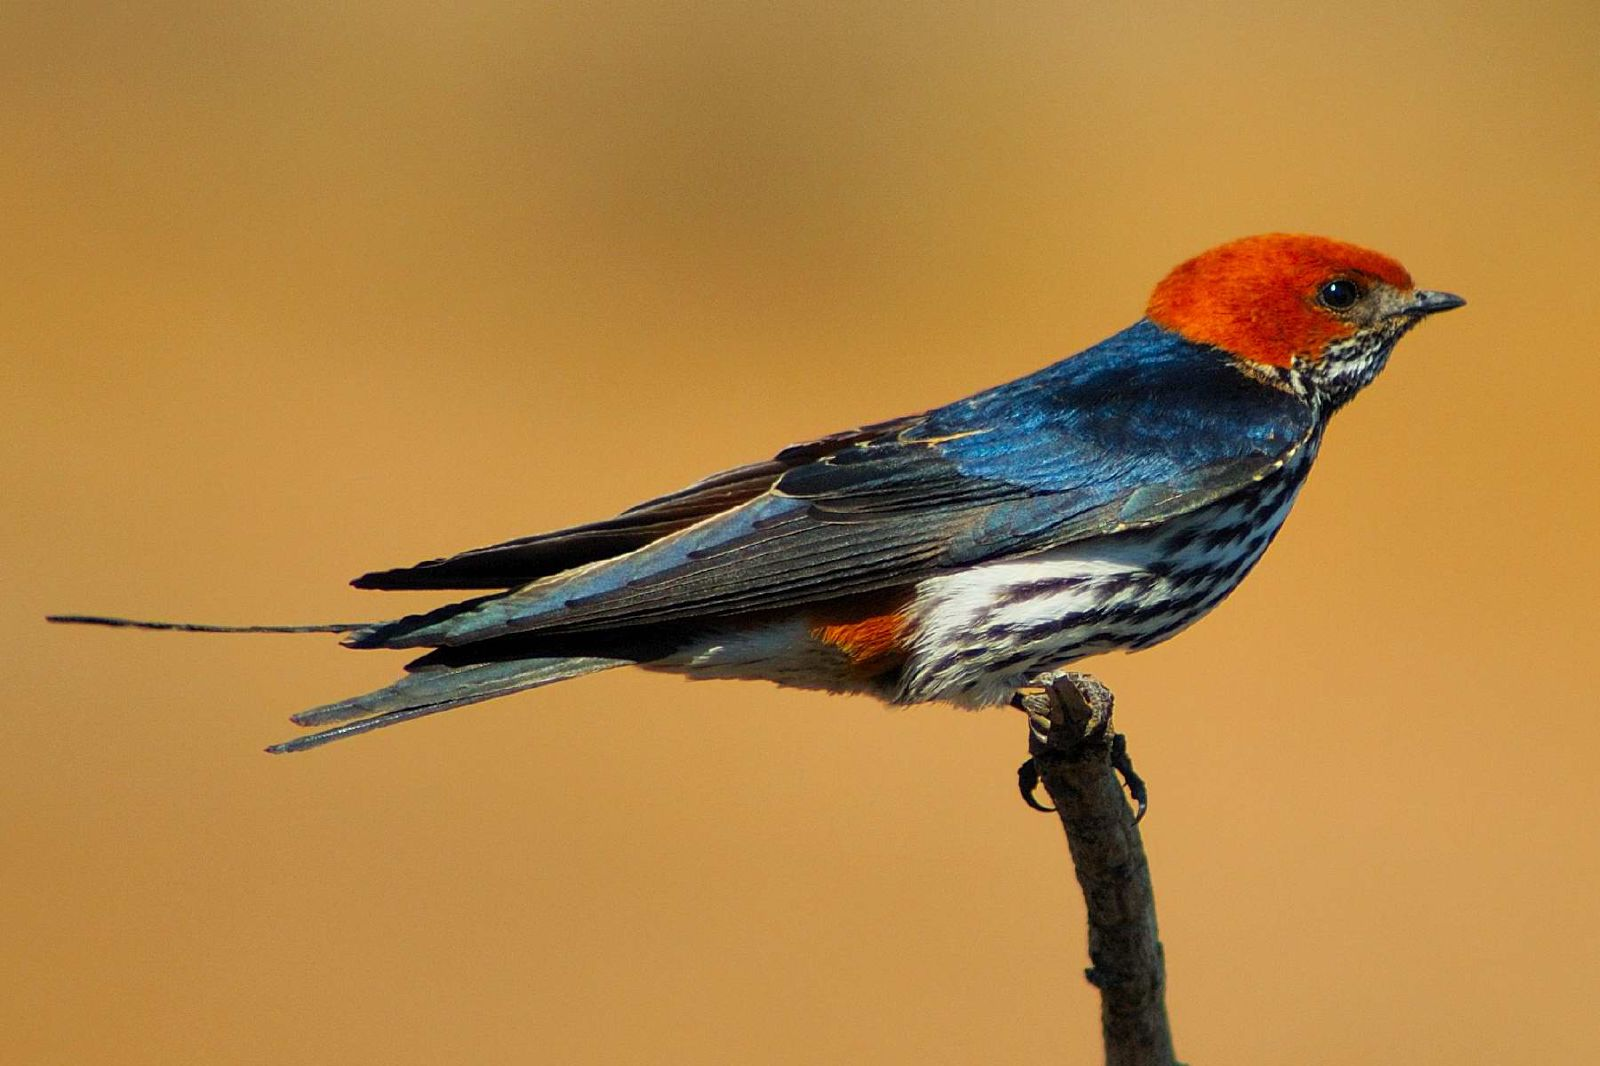
\includegraphics[width=0.5\columnwidth]{swallow.jpg} % Example image
\end{center}

\answer{While this question leaves out the crucial element of the geographic origin of the swallow, according to Jonathan Corum, an unladen European swallow maintains a cruising airspeed velocity of \textbf{11 metres per second}, or \textbf{24 miles an hour}. The velocity of the corresponding African swallows requires further research as kinematic data is severely lacking for these species.}

\end{question}

%----------------------------------------------------------------------------------------
%	QUESTION 2
%----------------------------------------------------------------------------------------

\begin{question}

\questiontext{How much wood would a woodchuck chuck if a woodchuck could chuck wood?}

%--------------------------------------------

\begin{subquestion}{Suppose ``chuck" implies throwing.} % Subquestion within question

\answer{According to the Associated Press (1988), a New York Fish and Wildlife technician named Richard Thomas calculated the volume of dirt in a typical 25--30 foot (7.6--9.1 m) long woodchuck burrow and had determined that if the woodchuck had moved an equivalent volume of wood, it could move ``about \textbf{700 pounds (320 kg)} on a good day, with the wind at his back".}

\end{subquestion}

%--------------------------------------------

\begin{subquestion}{Suppose ``chuck" implies vomiting.} % Subquestion within question

\answer{A woodchuck can ingest 361.92 cm\textsuperscript{3} (22.09 cu in) of wood per day. Assuming immediate expulsion on ingestion with a 5\% retainment rate, a woodchuck could chuck \textbf{343.82 cm\textsuperscript{3}} of wood per day.}

\end{subquestion}

%--------------------------------------------

\end{question}

%----------------------------------------------------------------------------------------
%	QUESTION 3
%----------------------------------------------------------------------------------------

\begin{question}

\questiontext{Identify the author of Equation \ref{eq:bayes} below and briefly describe it in English.}

\begin{equation}\label{eq:bayes}
	P(A|B) = \frac{P(B|A)P(A)}{P(B)}
\end{equation}

\answer{Lorem ipsum dolor sit amet, consectetur adipiscing elit. Praesent porttitor arcu luctus, imperdiet urna iaculis, mattis eros. Pellentesque iaculis odio vel nisl ullamcorper, nec faucibus ipsum molestie. Sed dictum nisl non aliquet porttitor. Etiam vulputate arcu dignissim, finibus sem et, viverra nisl. Aenean luctus congue massa, ut laoreet metus ornare in. Nunc fermentum nisi imperdiet lectus tincidunt vestibulum at ac elit. Nulla mattis nisl eu malesuada suscipit.}

\end{question}

%----------------------------------------------------------------------------------------

\assignmentSection{Bonus Questions}

%----------------------------------------------------------------------------------------
%	QUESTION 4
%----------------------------------------------------------------------------------------

\begin{question}

\questiontext{The table below shows the nutritional consistencies of two sausage types. Explain their relative differences given what you know about daily adult nutritional recommendations.}

\begin{table}[h]
	\centering % Centre the table
	\begin{tabular}{l l l}
		\toprule
		\textit{Per 50g} & Pork & Soy \\
		\midrule
		Energy & 760kJ & 538kJ\\
		Protein & 7.0g & 9.3g\\
		Carbohydrate & 0.0g & 4.9g\\
		Fat & 16.8g & 9.1g\\
		Sodium & 0.4g & 0.4g\\
		Fibre & 0.0g & 1.4g\\
		\bottomrule
	\end{tabular}
\end{table}

\answer{Lorem ipsum dolor sit amet, consectetur adipiscing elit. Praesent porttitor arcu luctus, imperdiet urna iaculis, mattis eros. Pellentesque iaculis odio vel nisl ullamcorper, nec faucibus ipsum molestie. Sed dictum nisl non aliquet porttitor. Etiam vulputate arcu dignissim, finibus sem et, viverra nisl. Aenean luctus congue massa, ut laoreet metus ornare in. Nunc fermentum nisi imperdiet lectus tincidunt vestibulum at ac elit. Nulla mattis nisl eu malesuada suscipit.}

\end{question}

%----------------------------------------------------------------------------------------
%	QUESTION 5
%----------------------------------------------------------------------------------------

\begin{question}

\lstinputlisting[
	caption=Luftballons Perl Script, % Caption above the listing
	label=lst:luftballons, % Label for referencing this listing
	language=Perl, % Use Perl functions/syntax highlighting
	frame=single, % Frame around the code listing
	showstringspaces=false, % Don't put marks in string spaces
	numbers=left, % Line numbers on left
	numberstyle=\tiny, % Line numbers styling
	]{luftballons.pl}

%--------------------------------------------

\begin{subquestion}{How many luftballons will be output by the Listing \ref{lst:luftballons} above?} % Subquestion within question

\answer{99 luftballons.}

\end{subquestion}

%--------------------------------------------

\begin{subquestion}{Identify the regular expression in Listing \ref{lst:luftballons} and explain how it relates to the anti-war sentiments found in the rest of the script.} % Subquestion within question

\answer{Lorem ipsum dolor sit amet, consectetur adipiscing elit. Praesent porttitor arcu luctus, imperdiet urna iaculis, mattis eros. Pellentesque iaculis odio vel nisl ullamcorper, nec faucibus ipsum molestie. Sed dictum nisl non aliquet porttitor. Etiam vulputate arcu dignissim, finibus sem et, viverra nisl. Aenean luctus congue massa, ut laoreet metus ornare in. Nunc fermentum nisi imperdiet lectus tincidunt vestibulum at ac elit. Nulla mattis nisl eu malesuada suscipit.}

\end{subquestion}

%--------------------------------------------

\end{question}

%----------------------------------------------------------------------------------------

\end{document}
